% !TEX TS-program = pdflatex
% !TEX encoding = UTF-8 Unicode

\documentclass{beamer}

\mode<presentation>
{
  \usetheme{Warsaw}
  % or ...

  \setbeamercovered{transparent}
  % or whatever (possibly just delete it)
}


\usepackage[english]{babel}
% or whatever
\usepackage{graphicx}

\usepackage[utf8]{inputenc}
% or whatever

\usepackage{times}
\usepackage[T1]{fontenc}
% Or whatever. Note that the encoding and the font should match. If T1
% does not look nice, try deleting the line with the fontenc.


\title[Short Paper Title] % (optional, use only with long paper titles)
{Critical states of slow pattern in neuronal networks}

%\subtitle
%{Include Only If Paper Has a Subtitle}

\author[Author, Another] % (optional, use only with lots of authors)
{Longbin Zeng\inst{1} \and S.~Another\inst{2}}
% - Give the names in the same order as the appear in the paper.
% - Use the \inst{?} command only if the authors have different
%   affiliation.

\institute[Universities of Somewhere and Elsewhere] % (optional, but mostly needed)
{
  \inst{1}%
  Department of Computer Science\\
  University of Somewhere
  \and
  \inst{2}%
  Department of Theoretical Philosophy\\
  University of Elsewhere}
% - Use the \inst command only if there are several affiliations.
% - Keep it simple, no one is interested in your street address.

\date[CFP 2003] % (optional, should be abbreviation of conference name)
{Conference on Fabulous Presentations, 2003}
% - Either use conference name or its abbreviation.
% - Not really informative to the audience, more for people (including
%   yourself) who are reading the slides online

\subject{Theoretical Computer Science}
% This is only inserted into the PDF information catalog. Can be left
% out. 



% If you have a file called "university-logo-filename.xxx", where xxx
% is a graphic format that can be processed by latex or pdflatex,
% resp., then you can add a logo as follows:

% \pgfdeclareimage[height=0.5cm]{university-logo}{university-logo-filename}
% \logo{\pgfuseimage{university-logo}}



% Delete this, if you do not want the table of contents to pop up at
% the beginning of each subsection:
\AtBeginSubsection[]
{
  \begin{frame}<beamer>{Outline}
    \tableofcontents[currentsection,currentsubsection]
  \end{frame}
}


% If you wish to uncover everything in a step-wise fashion, uncomment
% the following command: 

%\beamerdefaultoverlayspecification{<+->}


\begin{document}

\begin{frame}
  \titlepage
\end{frame}

\begin{frame}{Outline}
  \tableofcontents
  % You might wish to add the option [pausesections]
\end{frame}


% Structuring a talk is a difficult task and the following structure
% may not be suitable. Here are some rules that apply for this
% solution: 

% - Exactly two or three sections (other than the summary).
% - At *most* three subsections per section.
% - Talk about 30s to 2min per frame. So there should be between about
%   15 and 30 frames, all told.

% - A conference audience is likely to know very little of what you
%   are going to talk about. So *simplify*!
% - In a 20min talk, getting the main ideas across is hard
%   enough. Leave out details, even if it means being less precise than
%   you think necessary.
% - If you omit details that are vital to the proof/implementation,
%   just say so once. Everybody will be happy with that.

\section{Motivation}

\subsection{The Basic Problem That We Studied}

\begin{frame}{Network Dynamics}  % {Subtitles are optional.}
  % - A title should summarize the slide in an understandable fashion
  %   for anyone how does not follow everything on the slide itself.

  \begin{itemize}
  \item
    Network response correspond to specific neuronal parameter, including fire rate, degree of irregularity, spatiotemporal patterns in neuronal spike trains and neuronal critical dynamics.
  \item
	Explor the influence of simulation size of neuronal network as well as the community stuctural network. 2000, 5000, 10000, ..., 100 million. 
  \item 
  Synapase density and input heterogeneity.(to be confirmed)
  \end{itemize}
\end{frame}



\begin{frame}{Theoretical explanation}

  Mainly three aspects\ldots
  \begin{itemize}
  \item Explain the mechanism underly the trainsition dynamics.
    \begin{itemize}
    \item 
    input current variablity analysis.
    \item
      Mean-filed equation and hopf bifuraction
    \item    
      The real part of fixed point is decreasing.
    \end{itemize}
  \item
   fit the network response with a simple f unction.
  \end{itemize}
\end{frame}


\subsection{Previous Work}

\begin{frame}{Make Titles Informative.}
\end{frame}

\begin{frame}{Make Titles Informative.}
\end{frame}



\section{Our Results/Contribution}

\subsection{Main Results}

\begin{frame}{Criticality in large-scale network}
	Fit to function $ s\cdot tanh(ax+by+c) + t $
	\begin{itemize}
		\item in the small blcok, slop is $1.6$
		\item in the large-scale block, slop is $1.4$
	\end{itemize}
\begin{figure}[htbp]
	\centering
	\begin{minipage}{0.49\linewidth}
		\centering
		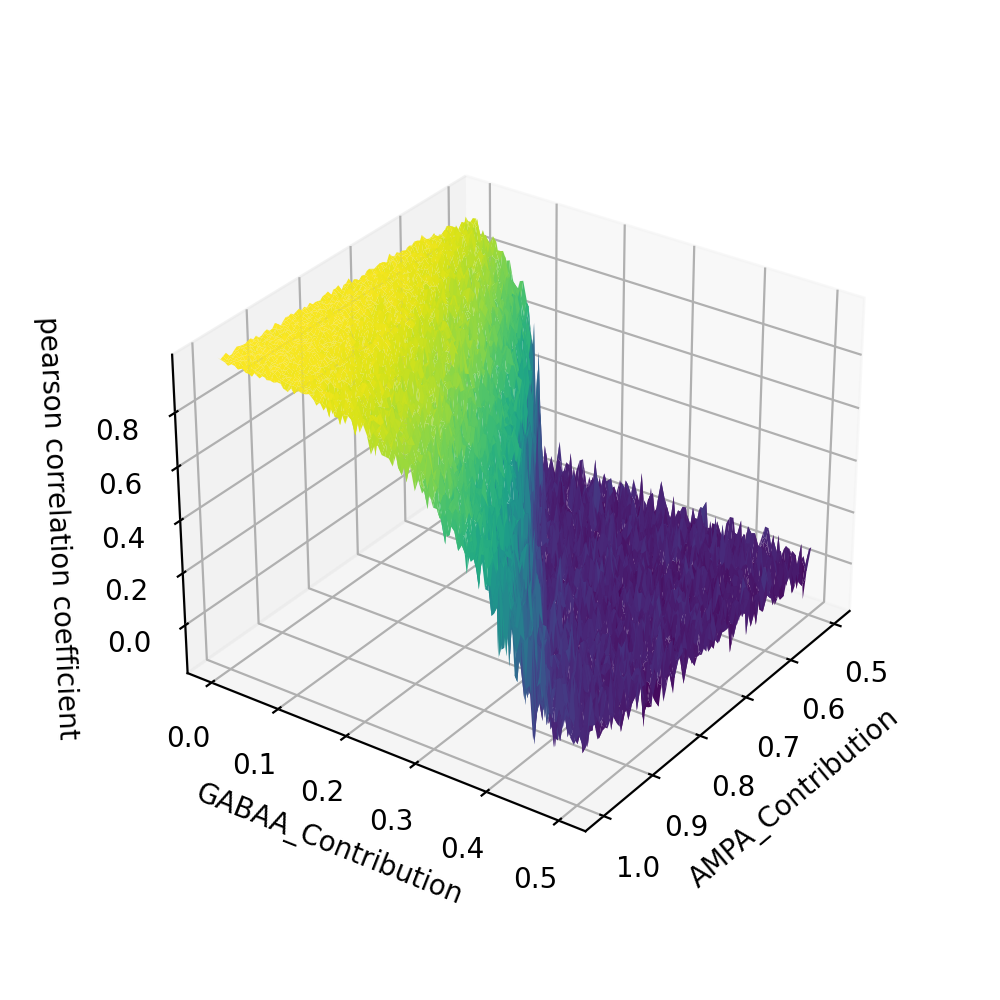
\includegraphics[width=0.9\linewidth]{../notebook/small_block_dense_grid_pcc}
		\caption{size=2k}
		\label{small_block}
	\end{minipage}
	%\qquad
	\begin{minipage}{0.49\linewidth}
		\centering
		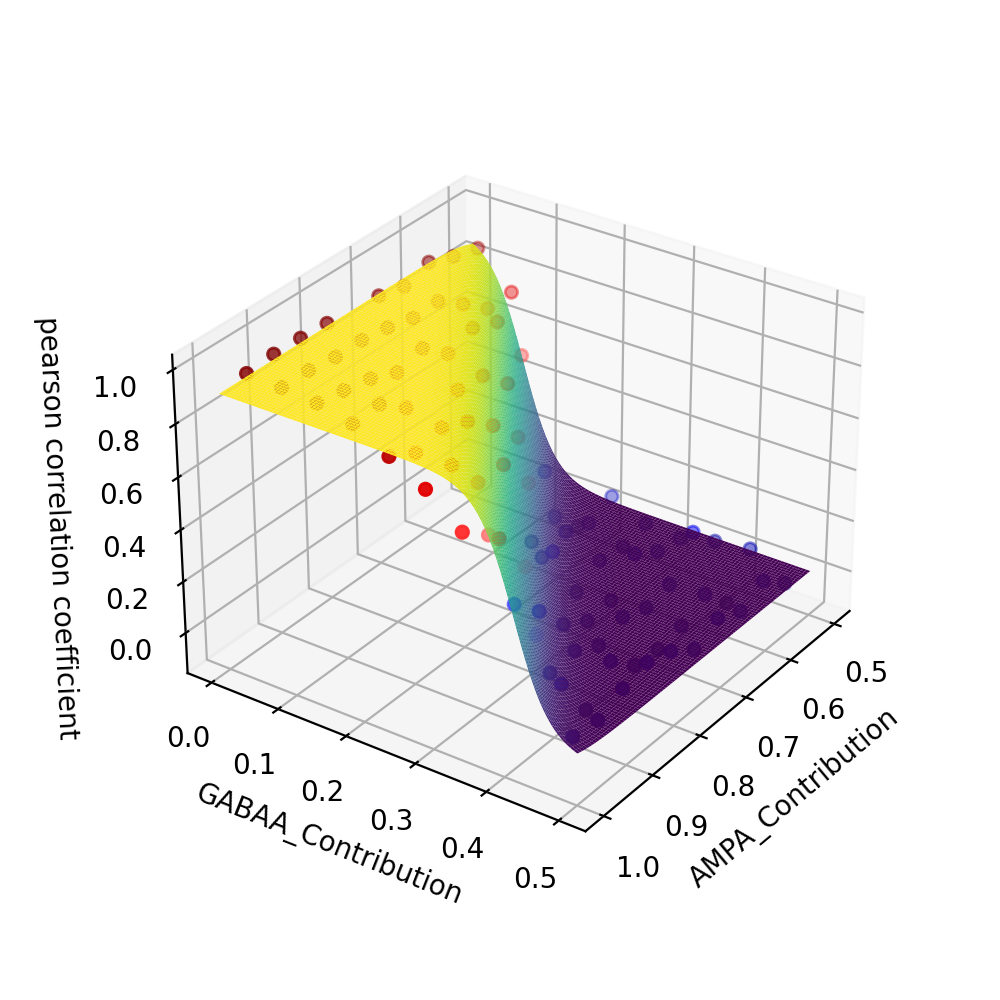
\includegraphics[width=0.9\linewidth]{../notebook/100m_block_sparse_point_pcc}
		\caption{size=100m}
		\label{big_block}
	\end{minipage}
\end{figure}
\end{frame}

\begin{frame}{Criticality in large-scale network}
	Some simulation case from a fixed parameter of critical space.
	\begin{figure}[htbp]
		\centering
		\begin{minipage}{0.49\linewidth}
			\centering
			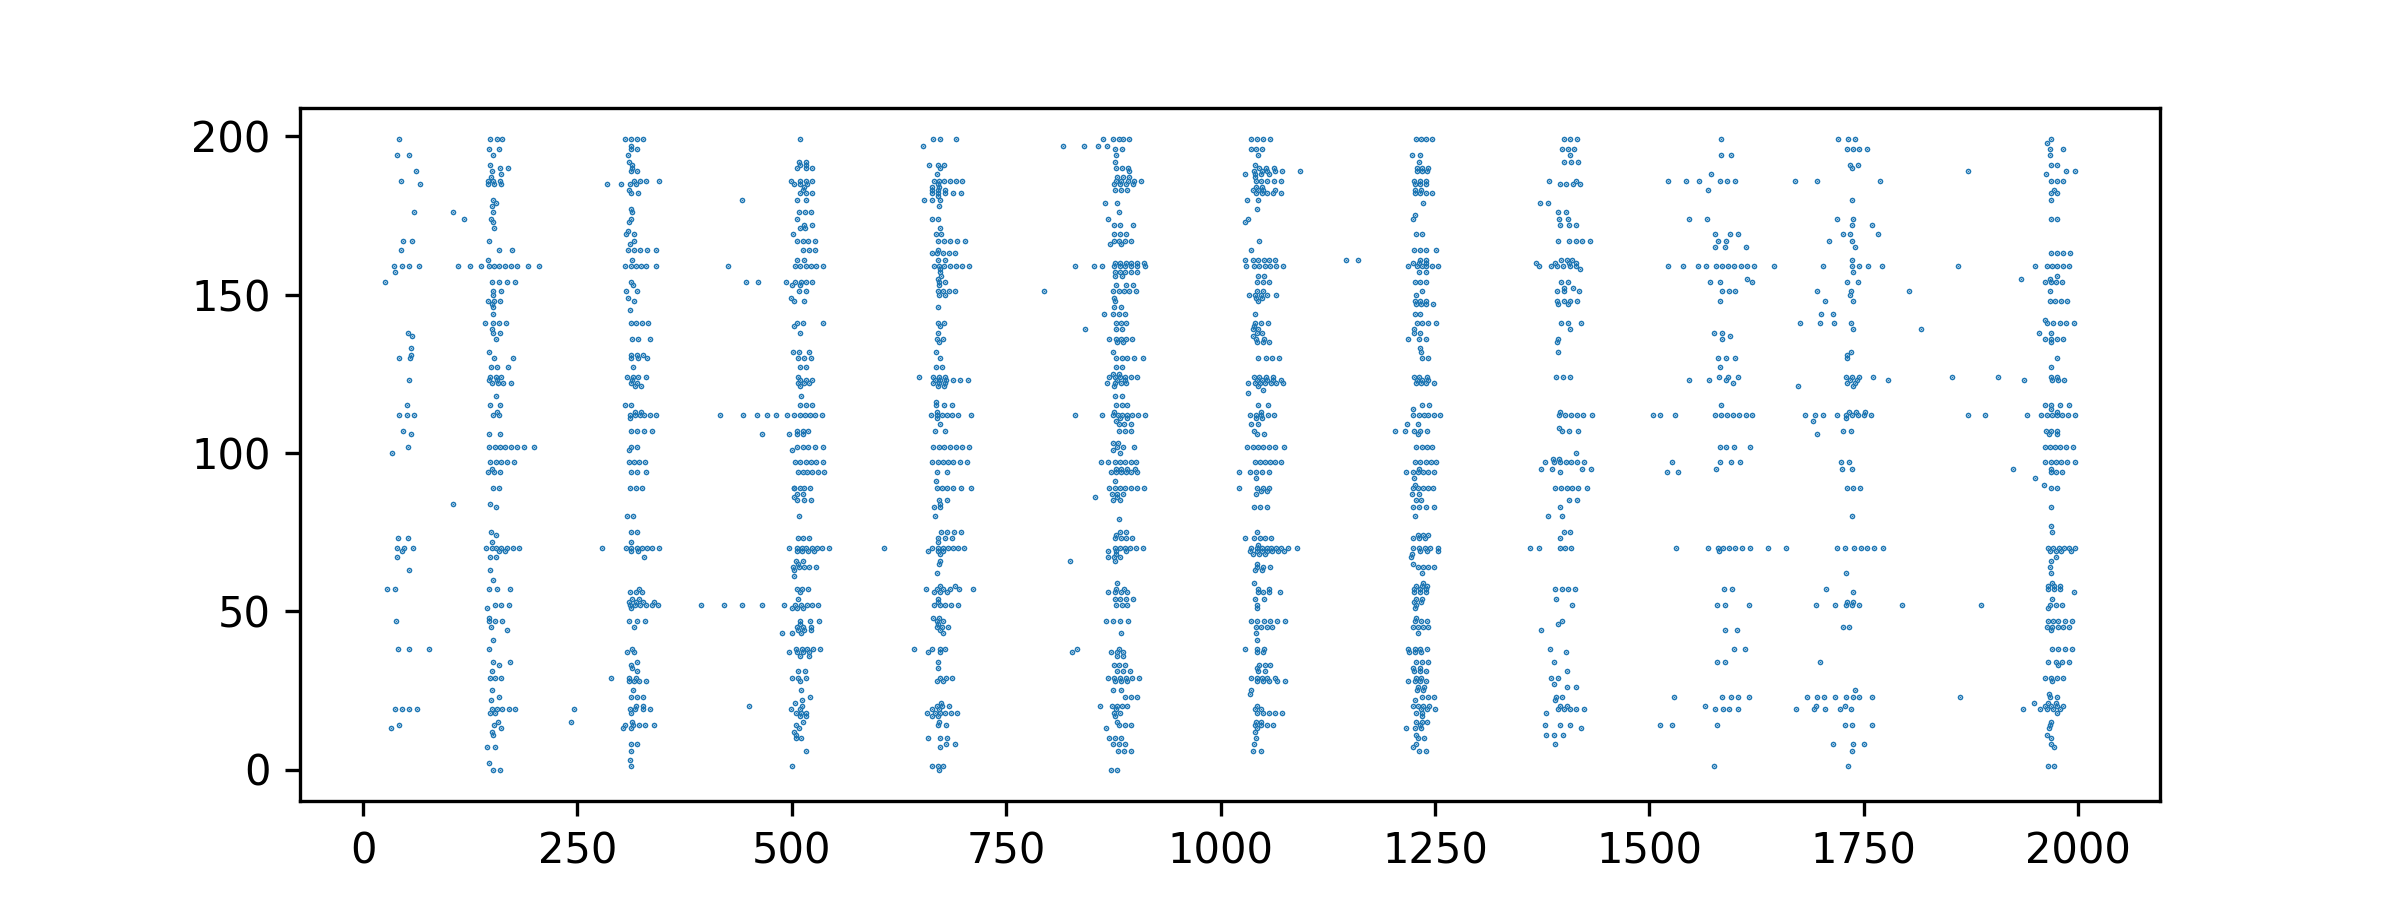
\includegraphics[width=0.9\linewidth]{fig/from_critical_size_10k}
			\caption{size=10k}
			\label{small_block}
		\end{minipage}
		%\qquad
		\begin{minipage}{0.49\linewidth}
			\centering
			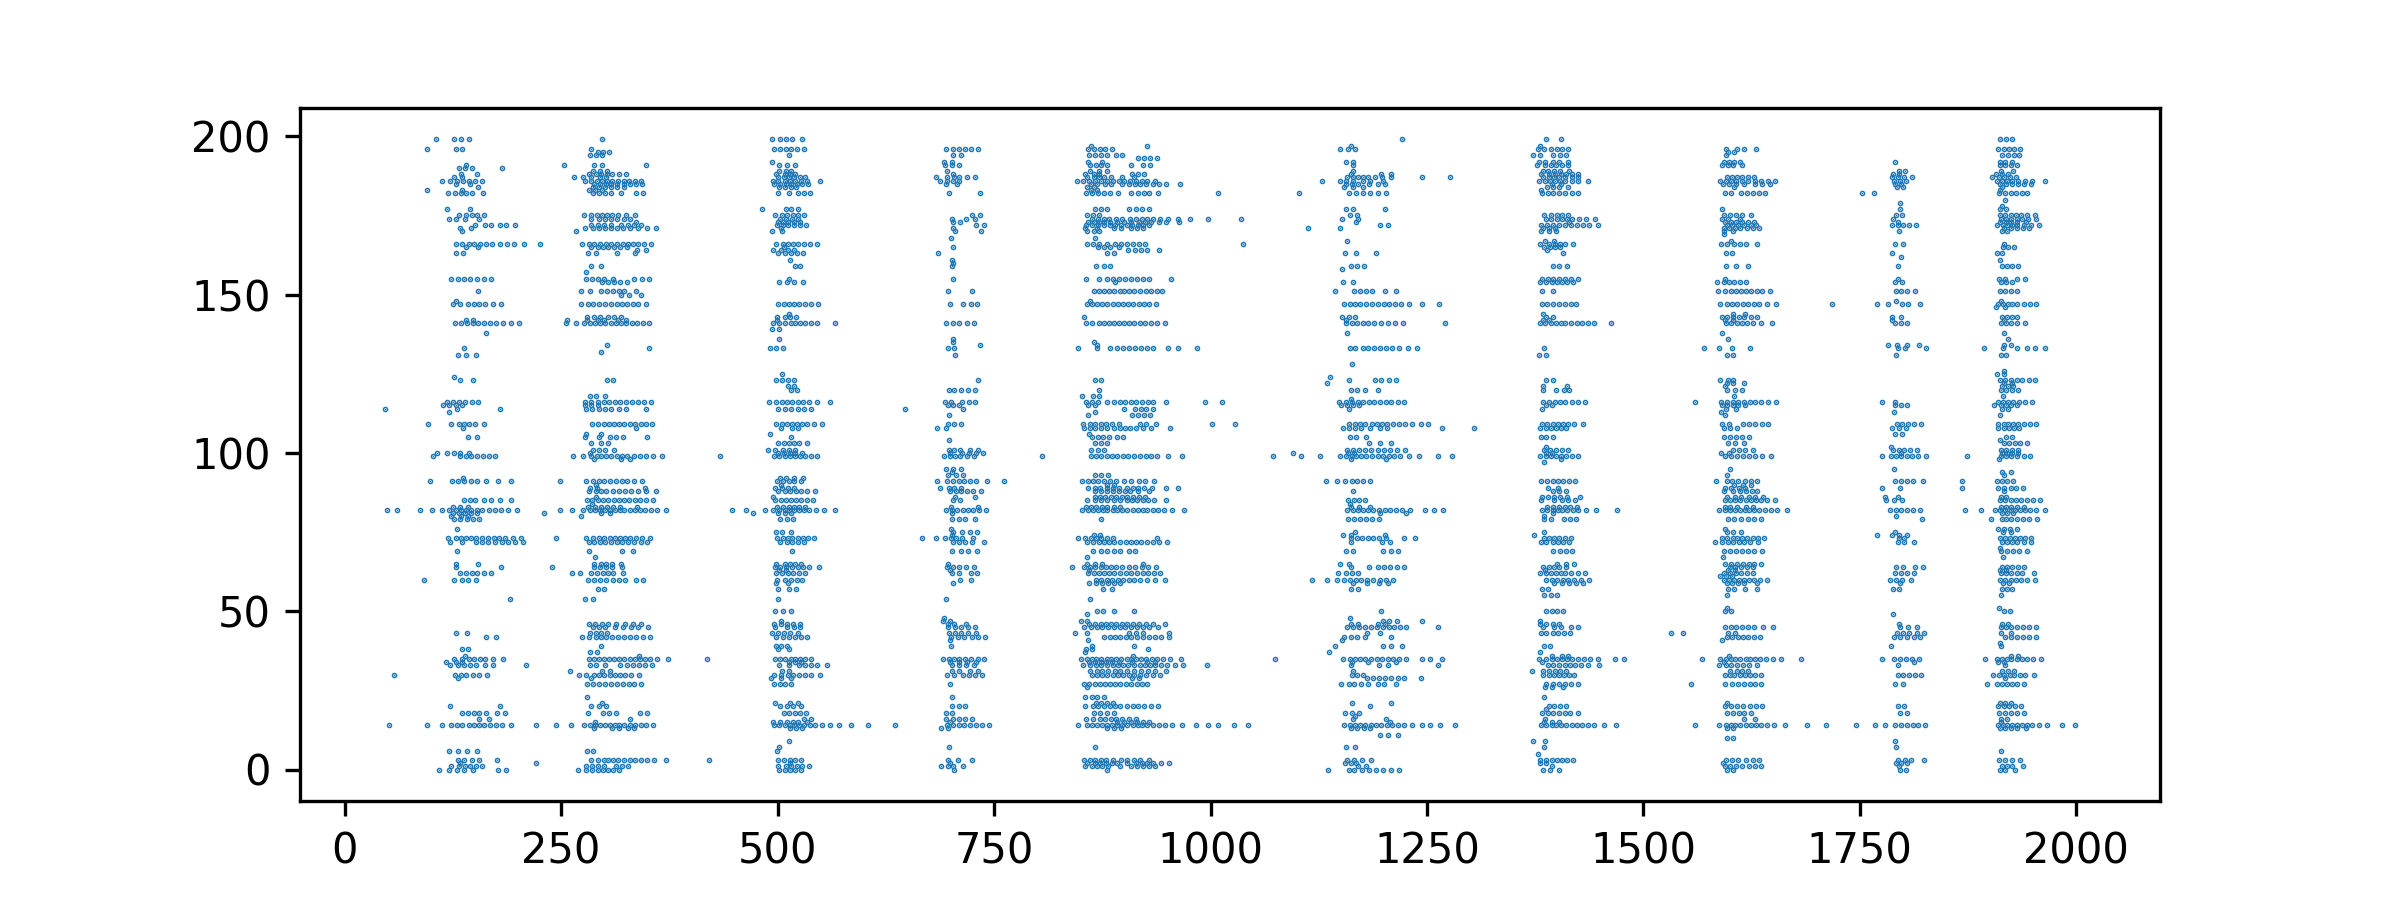
\includegraphics[width=0.9\linewidth]{fig/from_critical_size_100m}
			\caption{size=100m}
			\label{big_block}
		\end{minipage}
	\end{figure}
\end{frame}

\begin{frame}{Make Titles Informative.}
\end{frame}


\subsection{Basic Ideas for Proofs/Implementation}

\begin{frame}{Make Titles Informative.}
\end{frame}

\begin{frame}{Make Titles Informative.}
\end{frame}

\begin{frame}{Make Titles Informative.}
\end{frame}



\section*{Summary}

\begin{frame}{Summary}

  % Keep the summary *very short*.
  \begin{itemize}
  \item
    The \alert{first main message} of your talk in one or two lines.
  \item
    The \alert{second main message} of your talk in one or two lines.
  \item
    Perhaps a \alert{third message}, but not more than that.
  \end{itemize}
  
  % The following outlook is optional.
  \vskip0pt plus.5fill
  \begin{itemize}
  \item
    Outlook
    \begin{itemize}
    \item
      Something you haven't solved.
    \item
      Something else you haven't solved.
    \end{itemize}
  \end{itemize}
\end{frame}



% All of the following is optional and typically not needed. 
\appendix
\section<presentation>*{\appendixname}
\subsection<presentation>*{For Further Reading}

\begin{frame}[allowframebreaks]
  \frametitle<presentation>{For Further Reading}
    
  \begin{thebibliography}{10}
    
  \beamertemplatebookbibitems
  % Start with overview books.

  \bibitem{Author1990}
    A.~Author.
    \newblock {\em Handbook of Everything}.
    \newblock Some Press, 1990.
 
    
  \beamertemplatearticlebibitems
  % Followed by interesting articles. Keep the list short. 

  \bibitem{Someone2000}
    S.~Someone.
    \newblock On this and that.
    \newblock {\em Journal of This and That}, 2(1):50--100,
    2000.
  \end{thebibliography}
\end{frame}

\end{document}


